\section{Parameters}
\label{app:params}
Table \ref{tab:params} lists all parameters of BatSLAM 2.0. They are the default values of \texttt{batslam/config.py} in the accompanying code, and were used for all worlds, routes and sensors; none of them was tuned per test case.

\begin{table*}[t]
\centering
\footnotesize
\caption{Parameters of BatSLAM 2.0. The same values were used for every experiment in this paper.}
\label{tab:params}
\resizebox{\textwidth}{!}{\begin{tabular}{lll}
\toprule
Stage & Parameter & Value \\
\midrule
Front-end & Filterbank & 64 Gaussian bands, \SIrange{30}{90}{\kilo\hertz}, log-spaced, width of two band spacings \\
 & Band pooling & Pairs of bands (32 bands) \\
 & Range bins & \SI{6}{\centi\meter}, from \SI{0.25}{\meter} to \SI{10}{\meter} (162 bins) \\
 & Time-varying gain & Amplitude $\times r$ \\
 & Energy image & Cube root of the amplitude, relative to the peak of the view \\
 & Spectral-shape image & $\pm$\SI{15}{\deci\bel} scaled to $\pm 1$, only above \SI{-40}{\deci\bel} \\
 & Range smoothing & Gaussian, one bin (\SI{6}{\centi\meter}) \\
Templates & Spacing & \SI{0.45}{\meter} travelled or \SI{20}{\degree} turned \\
 & Range-shift search & $\pm 3$ bins ($\pm$\SI{18}{\centi\meter}) \\
 & Candidates & 5 per pulse, similarity $\ge \Smin$ \\
 & Exclusion of recent templates & \SI{6}{\meter} of travel \\
 & Heading gate & \SI{69}{\degree} (\SI{1.2}{\radian}) \\
Verifier & Evidence per match & $\LLRslope \cdot (s - \LLRmid)$, clipped to $\pm 4$ \\
 & Missed pulse & Penalty 0.5, dies after 4 missed pulses \\
 & Consistency & \SI{0.30}{\meter} $+ 0.15 \times$ distance, \SI{0.25}{\radian} \\
 & Commit & 8 pairs, 3 templates, evidence 10, margin 4 over rivals ($>$\SI{1}{\meter} or $>$\SI{0.4}{\radian} apart) \\
 & Plausibility gate & $\chi^2_3$ at 99.9\,\% (16.27); relative covariance for corrections $>$\SI{1.5}{\meter} \\
 & Risk-scaled commit & Correction $>$\SI{1.5}{\meter}: 16 pairs, evidence 40, evidence $\ge$ number of pairs \\
Pose graph & Prior & $\sigma = (0.01, 0.01, 0.005)$ \\
 & Odometry & $\sigma = (0.04, 0.02, 0.035) \cdot \sqrt{d} + (0.005, 0.005, 0.003)$ \\
 & Loop closure link & $\sigma = (0.30, 0.30, 0.20)$, Huber loss with threshold 1.345 \\
 & Solver & iSAM2, Dogleg, relinearization threshold 0.01 \\
Link management & Length rule & Fewer than 16 links after 10 pulses without a new link \\
 & Residual check & Median $\chi^2 > 12$ (tentative groups) \\
 & GNC audit & Every 400 nodes, Geman-McClure loss, keep if mean weight $\ge 0.5$ \\
\bottomrule
\end{tabular}}
\end{table*}

\section{Reproducibility}
\label{app:repro}
All code, scene definitions and experiment definitions are available at \url{https://github.com/Cosys-Lab/BatSLAM2}. The simulator (section \ref{sec:setup}) is included as a copy under \texttt{sim/simulator}. An important note concerns the HRTF data: the HRTF file that we started from stores its directivity arrays in (elevation, azimuth, frequency) order, while the interpolation routine of the simulator assumed (azimuth, elevation, frequency). As both angle grids are identical ($-$\SI{90}{\degree} to \SI{90}{\degree} in steps of \SI{2.5}{\degree}), this went unnoticed at first, and it caused the simulated ears to point up and down instead of left and right (a reflector \SI{45}{\degree} to the side produced an interaural level difference of only \SI{0.2}{\deci\bel}, and a reflector \SI{30}{\degree} above the head one of \SI{14}{\deci\bel}). All results in this paper were produced with the corrected (transposed) HRTF, for which the same test gives \SI{18}{\deci\bel} and \SI{0}{\deci\bel}, respectively. The check is included as \texttt{sim/check\_hrtf\_orientation.m}.

The datasets are generated with \texttt{sim/generate\_dataset.m} (worlds, drives, echoes and odometry) and \texttt{sim/generate\_capture\_dataset.m} (the capture study). The experiments are defined in \texttt{suites/hc\_main.json}, \texttt{suites/hc\_ablation.json} and \texttt{suites/hc\_robustness.json}, and are run with \texttt{scripts/run\_suite.py}. The front-end studies are run with \texttt{scripts/bench\_descriptor.py}, \texttt{scripts/bench\_sensor.py} and \texttt{scripts/capture\_analysis.py}. All numbers and tables in this paper are generated from the results by \texttt{scripts/build\_paper\_generated.py}, and all figures by \texttt{scripts/paper\_figures.py}.

\section{Result tables}
\label{app:tables}
This appendix lists the numerical results that are discussed in the main text: single-view place recognition for the design choices of the descriptor (table \ref{tab:descriptor}), the results of the complete system per condition (table \ref{tab:main}), the ablations (table \ref{tab:ablation}) and the real-world results (table \ref{tab:real}).

\begin{table}[t]
\centering
\footnotesize
\caption{Single-view place recognition for the design choices of the descriptor, with the design sensor. All variants use 32 channels, \SI{6}{\centi\meter} range bins and the TVG. Our descriptor uses a cube-root compression. Best value per column in bold. ILD: interaural level difference.}
\label{tab:descriptor}
\begin{tabular}{lrrrr}
\toprule
 & \multicolumn{2}{c}{Indoor floor} & \multicolumn{2}{c}{City} \\
\cmidrule(lr){2-3}\cmidrule(lr){4-5}
Variant & Top-1 & AUC & Top-1 & AUC \\
\midrule
\multicolumn{5}{l}{\textit{Cues}} \\
Energy & 0.875 & 0.915 & 0.878 & 0.918 \\
Energy + shape \textbf{(ours)} & 0.913 & 0.945 & 0.888 & 0.938 \\
Energy + shape + ILD & 0.892 & \textbf{0.968} & 0.878 & \textbf{0.960} \\
\midrule
\multicolumn{5}{l}{\textit{Compression of the energy image (energy + shape)}} \\
Logarithm, floor \SI{-30}{\deci\bel} & 0.884 & 0.930 & 0.888 & 0.930 \\
Logarithm, floor \SI{-50}{\deci\bel} & \textbf{0.929} & 0.947 & 0.886 & 0.925 \\
Square root & 0.900 & 0.940 & \textbf{0.889} & 0.937 \\
Linear & 0.858 & 0.925 & 0.857 & 0.921 \\
\midrule
\multicolumn{5}{l}{\textit{Matching of the original BatSLAM}} \\
Logarithmic energy, floor \SI{-30}{\deci\bel} & 0.401 & 0.801 & 0.599 & 0.814 \\
Energy + shape & 0.793 & 0.901 & 0.802 & 0.889 \\
\bottomrule
\end{tabular}
\end{table}

\begin{table}[t]
\centering
\footnotesize
\caption{Results of BatSLAM 2.0 per condition (ranges over the runs). ATE: trajectory error of odometry and of BatSLAM 2.0, without and after rigid alignment; wrong: wrong committed hypotheses in the final graph, out of all committed hypotheses; coverage: fraction of true revisits with a correct link.}
\label{tab:main}
\begin{tabular}{lrrrrr}
\toprule
 & \multicolumn{3}{c}{ATE [m]} & & \\
\cmidrule(lr){2-4}
Condition (runs) & Odometry & Ours & Aligned & Wrong & Coverage \\
\midrule
Calibrated (6) & 4.2--11.1 & 0.47--1.91 & 0.18--0.46 & 0/230 & 0.79--0.84 \\
Residual bias (6) & 11.0--19.0 & 0.62--1.65 & 0.23--0.53 & 0/227 & 0.79--0.84 \\
Degraded sensors (3) & 7.5 & 0.52--1.79 & 0.25--0.81 & 1/106 & 0.67--0.74 \\
Uncalibrated (4) & 19.1--22.3 & 1.38--12.68 & 0.45--2.96 & 0/149 & 0.62--0.81 \\
\bottomrule
\end{tabular}
\end{table}

\begin{table}[t]
\centering
\footnotesize
\caption{Ablations over four standard cases (routes 3 and 5 with calibrated odometry, route 7 with a residual bias, and the city). ATE: mean over the cases; wrong: wrong committed hypotheses in the final graphs, summed over the cases. Naive: no sequence verification and no link management.}
\label{tab:ablation}
\setlength{\tabcolsep}{5pt}
\begin{tabular}{lrrr}
\toprule
Variant & ATE [m] & Wrong & Coverage \\
\midrule
\textbf{Full system (ours)} & 0.87 & 0 & 0.81 \\
\midrule
Naive & 18.90 & 364 & 0.72 \\
No sequence verification & 4.85 & 10 & 0.80 \\
\midrule
Original front-end (8 bands) & 1.54 & 0 & 0.73 \\
No time-varying gain & 2.53 & 3 & 0.72 \\
Energy image only & 1.38 & 8 & 0.74 \\
No range-shift search & 1.47 & 0 & 0.60 \\
Hand-set evidence constants & 1.51 & 0 & 0.68 \\
\midrule
No risk-scaled commit & 0.93 & 1 & 0.81 \\
Length only (24 pairs) & 1.20 & 0 & 0.81 \\
No link management & 0.55 & 0 & 0.82 \\
\bottomrule
\end{tabular}
\end{table}

\begin{table*}[t]
\centering
\caption{Real-world results, mean (standard deviation) over ten odometry seeds (distance $\times 0.95$, rotation $\times 1.10$).}
\label{tab:real}
% generated by real/build_paper_real.py - do not edit
\begin{tabular}{lrrrrrrr}
\toprule
Evidence curve & ATE & Aligned & Links & Precision & Wrong & Revisits & Collapsed \\
 & (\si{\meter}) & (\si{\meter}) & & & Hyp. & Linked & Pairs \\
\midrule
Odometry only & 3.62~(0.46) & & & & & & \\
Simulation evidence curve & 0.77~(0.07) & 0.60~(0.05) & 108 & 1.000~(0.000) & 0 & 0.50~(0.01) & 0.000 \\
Refitted, even stretches & 0.67~(0.13) & 0.52~(0.11) & 141 & 0.980~(0.018) & 0 & 0.64~(0.10) & 0.000 \\
Refitted, odd stretches & 0.66~(0.12) & 0.52~(0.11) & 142 & 0.975~(0.021) & 0 & 0.64~(0.10) & 0.000 \\
\bottomrule
\end{tabular}

\end{table*}

\clearpage
\section{Additional results}
\label{app:runs}
In this appendix, we show the trajectories and the detailed results of all runs of the main and robustness experiments, and of the ablations. In every map, the grey line is the ground truth, the orange line the dead-reckoning estimate, and the blue line the trajectory estimated by BatSLAM 2.0 (without alignment, as it was estimated online). Links of wrong committed hypotheses that remain in the final graph would be drawn in red. The title of every panel lists the trajectory error of BatSLAM 2.0 and of odometry, and the number of wrong committed hypotheses in the final graph.

\begin{figure*}[p]
\centering
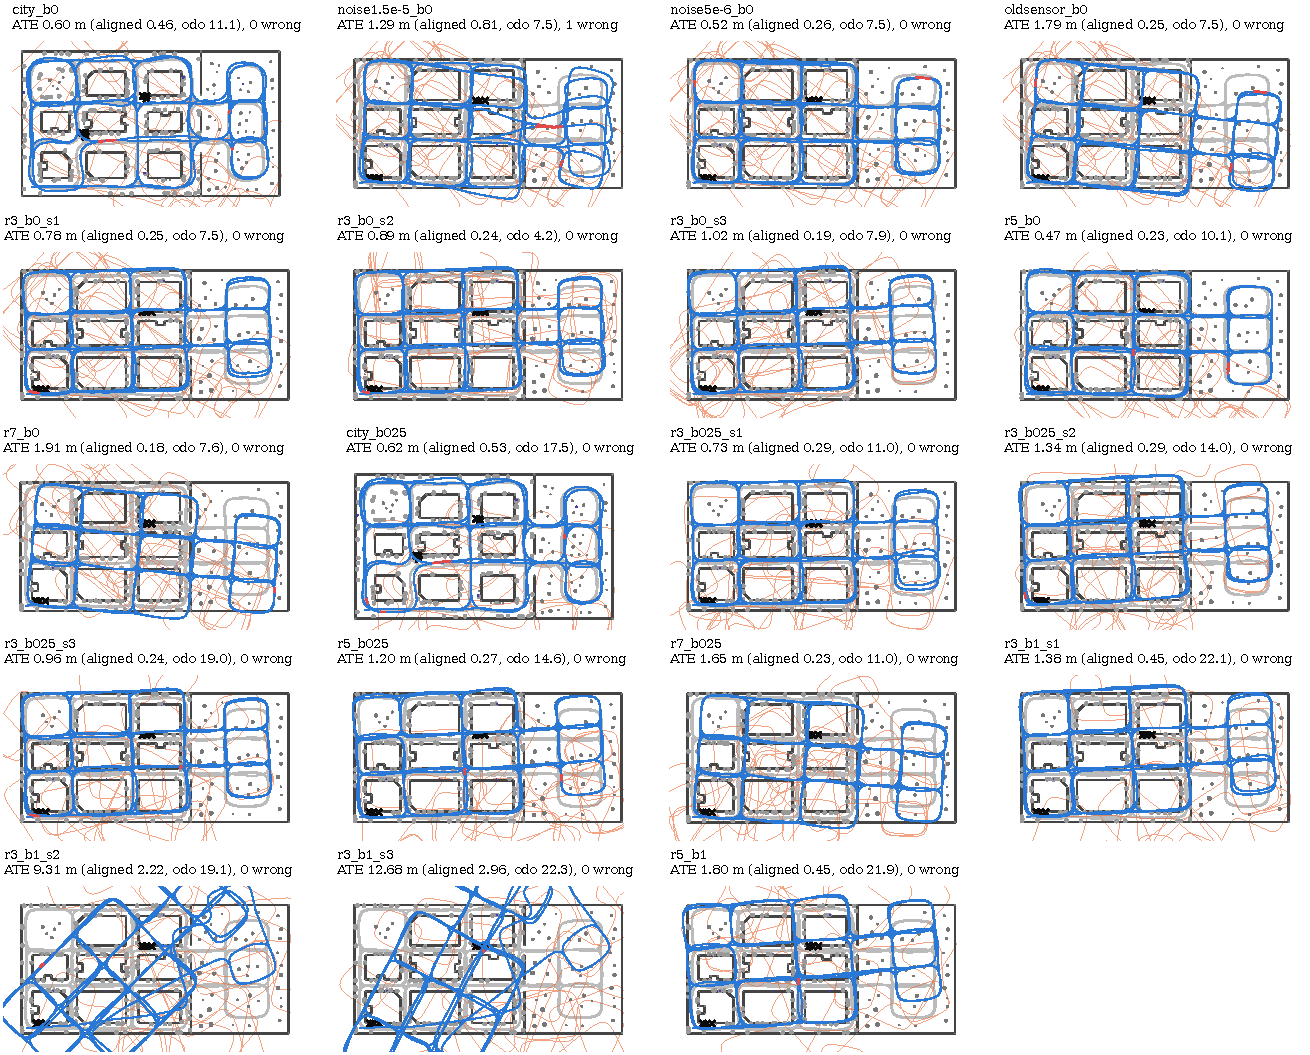
\includegraphics[width=\linewidth]{figures/appendixMaps_hc_main.pdf}
\caption{Trajectories of all runs of the main experiment (table \ref{tab:mainRuns}), sorted by the odometry condition. Grey: ground truth; orange: odometry; blue: BatSLAM 2.0. Run names: \texttt{r3}, \texttt{r5}, \texttt{r7}: routes 3, 5 and 7 on the indoor floor; \texttt{city}: the city world; \texttt{b0}, \texttt{b025}, \texttt{b1}: bias factor $b = 0$, $0.25$ and $1$; \texttt{s1}--\texttt{s3}: odometry noise realization; \texttt{noise5e-6}, \texttt{noise1.5e-5}, \texttt{oldsensor}: degraded sensors.}
\label{fig:appendixMaps}
\end{figure*}

\begin{figure*}[p]
\centering
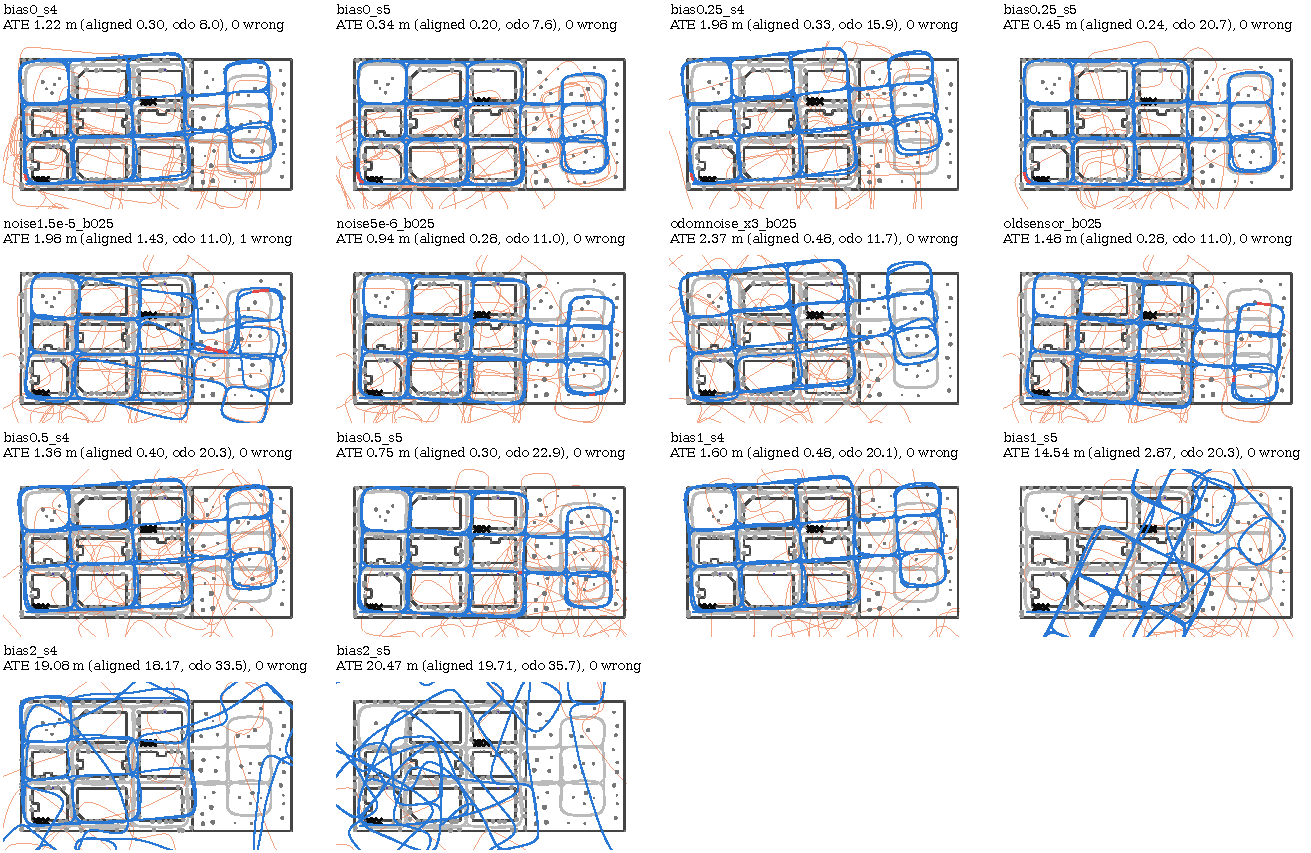
\includegraphics[width=\linewidth]{figures/appendixMaps_hc_robustness.pdf}
\caption{Trajectories of all runs of the robustness experiment (table \ref{tab:robustness}). \texttt{bias}$b$\texttt{\_s}$k$: bias factor $b$ with odometry realization $k$; \texttt{odomnoise\_x3}: three times the random odometry noise; the last three runs use degraded sensors with a residual bias. Colors as in figure \ref{fig:appendixMaps}.}
\label{fig:appendixMapsRobust}
\end{figure*}

\begin{table*}[htbp]
\centering
\footnotesize
\caption{Results of BatSLAM 2.0 on all runs of the main experiment (drives of about \SI{1}{\kilo\meter}). ATE odo: dead reckoning; ATE and aligned: BatSLAM 2.0 without and after rigid alignment; precision: fraction of correct links; wrong (final / all): wrong committed hypotheses in the final graph and over all commits; coverage: fraction of true revisits with a correct link; collapsed: fraction of collapsed pairs.}
\label{tab:mainRuns}
\resizebox{\linewidth}{!}{\begin{tabular}{llrrrrrrrr}
\toprule
Case & Odometry & ATE odo & ATE & Aligned & Precision & Wrong (final) & Wrong (all) & Coverage & Collapsed \\
 & & [m] $\downarrow$ & [m] $\downarrow$ & [m] $\downarrow$ & $\uparrow$ & $\downarrow$ & $\downarrow$ & $\uparrow$ & [\%] $\downarrow$ \\
\midrule
Indoor, route 3, seed 1 & Calibrated & 7.5 & \textbf{0.78} & 0.25 & 0.999 & 0/39 & 0 & 0.84 & 0.0 \\
Indoor, route 3, seed 2 & Calibrated & 4.2 & \textbf{0.89} & 0.24 & 0.999 & 0/40 & 0 & 0.84 & 0.0 \\
Indoor, route 3, seed 3 & Calibrated & 7.9 & \textbf{1.02} & 0.19 & 1.000 & 0/36 & 1 & 0.84 & 0.0 \\
Indoor, route 5 & Calibrated & 10.1 & \textbf{0.47} & 0.23 & 0.998 & 0/45 & 0 & 0.82 & 0.0 \\
Indoor, route 7 & Calibrated & 7.6 & \textbf{1.91} & 0.18 & 1.000 & 0/46 & 0 & 0.80 & 0.0 \\
City & Calibrated & 11.1 & \textbf{0.60} & 0.46 & 0.996 & 0/24 & 0 & 0.79 & 0.0 \\
Indoor, route 3, sensor $-10$~dB & Calibrated & 7.5 & \textbf{0.52} & 0.26 & 0.997 & 0/34 & 0 & 0.72 & 0.0 \\
Indoor, route 3, sensor $-20$~dB & Calibrated & 7.5 & \textbf{1.29} & 0.81 & 0.989 & 1/32 & 2 & 0.67 & 0.1 \\
Indoor, route 3, original sensor & Calibrated & 7.5 & \textbf{1.79} & 0.25 & 0.995 & 0/40 & 3 & 0.74 & 0.0 \\
\midrule
Indoor, route 3, seed 1 & Residual bias & 11.0 & \textbf{0.73} & 0.29 & 1.000 & 0/38 & 1 & 0.83 & 0.0 \\
Indoor, route 3, seed 2 & Residual bias & 14.0 & \textbf{1.34} & 0.29 & 1.000 & 0/38 & 0 & 0.84 & 0.0 \\
Indoor, route 3, seed 3 & Residual bias & 19.0 & \textbf{0.96} & 0.24 & 0.999 & 0/40 & 1 & 0.84 & 0.0 \\
Indoor, route 5 & Residual bias & 14.6 & \textbf{1.20} & 0.27 & 0.999 & 0/41 & 0 & 0.80 & 0.0 \\
Indoor, route 7 & Residual bias & 11.0 & \textbf{1.65} & 0.23 & 1.000 & 0/42 & 0 & 0.79 & 0.0 \\
City & Residual bias & 17.5 & \textbf{0.62} & 0.53 & 0.994 & 0/28 & 0 & 0.82 & 0.0 \\
\midrule
Indoor, route 3, seed 1 & Uncalibrated & 22.1 & \textbf{1.38} & 0.45 & 1.000 & 0/37 & 1 & 0.81 & 0.0 \\
Indoor, route 3, seed 2 & Uncalibrated & 19.1 & \textbf{9.31} & 2.22 & 0.998 & 0/36 & 1 & 0.62 & 0.6 \\
Indoor, route 3, seed 3 & Uncalibrated & 22.3 & \textbf{12.68} & 2.96 & 0.999 & 0/33 & 1 & 0.62 & 0.8 \\
Indoor, route 5 & Uncalibrated & 21.9 & \textbf{1.80} & 0.45 & 1.000 & 0/43 & 0 & 0.75 & 0.0 \\
\bottomrule
\end{tabular}
}
\end{table*}

\begin{table*}[htbp]
\centering
\footnotesize
\caption{Robustness runs: odometry bias factor $b$, three times the random odometry noise, and degraded sensors with a residual bias. Columns as in table \ref{tab:mainRuns}.}
\label{tab:robustness}
\resizebox{\linewidth}{!}{\begin{tabular}{llrrrrrrrr}
\toprule
Case & Bias & ATE odo & ATE & Aligned & Precision & Wrong (final) & Wrong (all) & Coverage & Collapsed \\
 & & [m] $\downarrow$ & [m] $\downarrow$ & [m] $\downarrow$ & $\uparrow$ & $\downarrow$ & $\downarrow$ & $\uparrow$ & [\%] $\downarrow$ \\
\midrule
Indoor, route 3, seed 4 & $b = 0$ & 8.0 & \textbf{1.22} & 0.30 & 1.000 & 0/38 & 1 & 0.82 & 0.0 \\
Indoor, route 3, seed 5 & $b = 0$ & 7.6 & \textbf{0.34} & 0.20 & 0.999 & 0/40 & 1 & 0.83 & 0.0 \\
Indoor, route 3, seed 4 & $b = 0.25$ & 15.9 & \textbf{1.98} & 0.33 & 0.999 & 0/38 & 1 & 0.83 & 0.0 \\
Indoor, route 3, seed 5 & $b = 0.25$ & 20.7 & \textbf{0.45} & 0.24 & 0.999 & 0/37 & 2 & 0.83 & 0.0 \\
Indoor, route 3, sensor $-20$~dB & $b = 0.25$ & 11.0 & \textbf{1.98} & 1.43 & 0.988 & 1/33 & 3 & 0.65 & 0.2 \\
Indoor, route 3, sensor $-10$~dB & $b = 0.25$ & 11.0 & \textbf{0.94} & 0.28 & 1.000 & 0/37 & 2 & 0.76 & 0.0 \\
Indoor, route 3, seed 1, odometry noise $\times 3$ & $b = 0.25$ & 11.7 & \textbf{2.37} & 0.48 & 1.000 & 0/50 & 1 & 0.81 & 0.0 \\
Indoor, route 3, original sensor & $b = 0.25$ & 11.0 & \textbf{1.48} & 0.28 & 0.998 & 0/38 & 2 & 0.73 & 0.0 \\
Indoor, route 3, seed 4 & $b = 0.5$ & 20.3 & \textbf{1.36} & 0.40 & 1.000 & 0/38 & 1 & 0.82 & 0.0 \\
Indoor, route 3, seed 5 & $b = 0.5$ & 22.9 & \textbf{0.75} & 0.30 & 1.000 & 0/40 & 1 & 0.82 & 0.0 \\
Indoor, route 3, seed 4 & $b = 1$ & 20.1 & \textbf{1.60} & 0.48 & 1.000 & 0/40 & 1 & 0.83 & 0.0 \\
Indoor, route 3, seed 5 & $b = 1$ & 20.3 & \textbf{14.54} & 2.87 & 1.000 & 0/32 & 1 & 0.62 & 0.8 \\
Indoor, route 3, seed 4 & $b = 2$ & 33.5 & \textbf{19.08} & 18.17 & 1.000 & 0/23 & 0 & 0.41 & 4.8 \\
Indoor, route 3, seed 5 & $b = 2$ & 35.7 & \textbf{20.47} & 19.71 & 1.000 & 0/11 & 0 & 0.32 & 7.4 \\
\bottomrule
\end{tabular}
}
\end{table*}

\begin{table*}[htbp]
\centering
\footnotesize
\caption{Ablation of the safeguards on the four hardest cases (three degraded sensors and route 3 with odometry seed 3). Every cell lists the aligned trajectory error (m) and, in parentheses, the number of wrong hypotheses in the final graph; the last two columns sum the wrong hypotheses in the final graphs and over all commits.}
\label{tab:ablationHard}
\resizebox{\linewidth}{!}{\begin{tabular}{lrrrrrr}
\toprule
Variant & $-10$~dB sensor & $-20$~dB sensor & Original sensor & Route 3, seed 3 & Wrong (final) & Wrong (all) \\
\midrule
No risk-scaled commit & 0.26 (0) & 0.24 (0) & 1.06 (1) & 0.19 (0) & 1 & 10 \\
Risk-scaled commit, length only (24 pairs) & 0.26 (0) & 0.24 (0) & 0.25 (0) & 0.19 (0) & 0 & 5 \\
Plausibility gate on the absolute marginal & 0.26 (0) & 0.23 (0) & 0.69 (1) & 0.19 (0) & 1 & 12 \\
No plausibility gate & 0.26 (0) & 1.37 (2) & 0.60 (1) & 0.19 (0) & 3 & 19 \\
No length rule & 0.26 (0) & 0.81 (2) & 1.07 (3) & 0.20 (2) & 7 & 7 \\
No link management & 0.26 (0) & 0.81 (2) & 1.07 (3) & 0.20 (2) & 7 & 7 \\
\midrule
\textbf{Full system (ours)} & 0.26 (0) & 0.81 (1) & 0.25 (0) & 0.19 (0) & 1 & 6 \\
\bottomrule
\end{tabular}
}
\end{table*}

\begin{table*}[htbp]
\centering
\footnotesize
\caption{Ablations per case: trajectory error (ATE, in m) and the number of wrong committed hypotheses in the final graph (in parentheses), for route 3 and route 5 with calibrated odometry, route 7 with a residual bias, and the city with calibrated odometry.}
\label{tab:ablationCases}
\begin{tabular}{lrrrr}
\toprule
Variant & Route 3 & Route 5 & Route 7, residual bias & City \\
\midrule
Naive (single views, no gates, no link mgmt.) & 8.00 (63) & 26.70 (68) & 8.22 (72) & 32.68 (161) \\
No sequence verification (single views) & 5.08 (1) & 1.95 (1) & 8.17 (6) & 4.21 (2) \\
Original front-end (8 wide bands) & 1.97 (0) & 0.44 (0) & 3.15 (0) & 0.59 (0) \\
No time-varying gain & 0.85 (1) & 6.82 (2) & 1.84 (0) & 0.62 (0) \\
Energy image only (no shape) & 0.63 (0) & 1.70 (3) & 1.26 (4) & 1.92 (1) \\
No range-shift search & 0.45 (0) & 1.57 (0) & 3.28 (0) & 0.56 (0) \\
No risk-scaled commit & 0.88 (0) & 0.46 (0) & 1.79 (1) & 0.57 (0) \\
Risk-scaled commit, length only (24 pairs) & 0.74 (0) & 0.47 (0) & 2.98 (0) & 0.60 (0) \\
Risk-scaled commit, length only (16 pairs) & 0.78 (0) & 0.47 (0) & 1.78 (1) & 0.52 (0) \\
No length rule & 0.63 (0) & 0.47 (0) & 0.49 (0) & 0.63 (0) \\
No link management & 0.63 (0) & 0.47 (0) & 0.49 (0) & 0.63 (0) \\
No plausibility gate & 0.78 (0) & 0.47 (0) & 1.65 (0) & 0.60 (0) \\
Plausibility gate on the absolute marginal & 0.78 (0) & 0.47 (0) & 1.65 (0) & 0.60 (0) \\
No heading gate & 0.64 (0) & 0.42 (0) & 1.55 (0) & 0.50 (0) \\
Hand-set evidence constants & 0.68 (0) & 0.63 (0) & 3.29 (0) & 1.45 (0) \\
\midrule
\textbf{Full system (ours)} & 0.78 (0) & 0.47 (0) & 1.65 (0) & 0.60 (0) \\
\bottomrule
\end{tabular}

\end{table*}

